%%
%% Template Experiments.tex
%%

% \chapter{Experiments}
% \label{cha:Experiments}

\section{Experiments}
\label{sec:experiments}

We test our algorithm on a Ubuntu 16.04 LTS server, with 4 2.4GHz
Intel Xeon processors and 128GB memory. The Maxflow v$3.04$
library developed by \citename{Kolmogorov:PAMI07} is used for
implementing the graph-cut algorithm. The cutting-plane algorithm
were performed using \citename{tsochantaridis2005large}'s
$\text{SVM}^{light}$ C++ library. We use Matlab R2016b's
quadratic programming engine for solving our learning algorithm's
objective problem. Regular SVM training and testing is
implemented by scikit-learn's svm module.


\subsection{Dataset preparation and configuration}
\label{sec:exp_data}

Our use CSI 300's daily market price (open, high, low, close,
volume), from 1st Jan 2015 to 31st Dec 2016, as our fundamental
dataset. There are $246 + 245 = 491$ samples in total. We then
calculated our technical analysis indicators (MACD-5, MACD-10,
KDJ-9) basing on this dataset. We further processed our dataset
with studentized residual normalization. Finally those samples
were split into two collections: 394 samples for training set and
97 samples for testing purpose. Our data are collected from Wind
dataset. During training stage, we used leave-one-out 10-fold
cross-validation to avoid over-fitting. The penalization
parameter $C$ in equation~\eqref{eq:ssvm_objective} was set to
$0.001$.

\subsection{Comparsion with SVM}
\label{sec:exp_compare}

\begin{table}
  \normalsize
  \centering
  \begin{tabular}{|l|c|c|}
    \hline
    {\sc Model} & {\sc Train Accuracy} & {\sc Test Accuracy}\\
    \hline \hline
    SSVM & 74.7\% & 63.1\% \\
    \hline
    SVM & 46.8\% & 22.6\% \\
    \hline
  \end{tabular}
  \caption{\label{tab:exp_compare} Results comparison
    between SSVM and SVM.}
\end{table}

From table~\ref{tab:exp_compare}, we can conclude that the train
accuracy and test accuracy of SSVM is better than that of SVM,
which proves that our model is better than the traditional
method.

\subsection{Real-world application}
\label{sec:exp_strategy}

According to the result of cluster analysis, the top 10 companies
which have the closest cooperation with other companies among the
CSI 300 are China Life Insurance Co., Sanan Optoelectronics,
Sinopec Group, Huadong Medicine Co., Shenzhen Inovance Technology
Co., Liaoning Cheng Da Co., Yongtai energy Limited by Share,
Wanxiang Qianchao Co., China Communications Construction Co., and
Bohai Financial Investment Holding Co.. All of these companies
are the industry leaders and they even have a great number of
hybrid businesses, especially the top 3 of them: Sinopec Group,
China Life Insurance Co. and Liaoning Cheng Da Co..

As the biggest chemical manufacturer in China and the No. 2
refiner in the world, the Sinopec Group has a series of
comparative advantages: its refining capacity accounts for half
of the China’s oil market share, and the distribution of its
refineries is close to the consumer market, resulting in its
strategic position. The complete pluralization and integration
and the balanced development of upriver and downstream lead to
its ability to fight fluctuation.

The controlling shareholder of China Life Insurance Co. is an
exclusive state-funded corporation. The strong background of
state-owned shareholder offers abundant of customer resource and
great financial investment platform. Recently, the China Life
Insurance Co. have reached strategic partnerships with many local
governments and famous enterprises. When the industry enters
differentiation phase, the position of industry leader shows up.
In 2016, Liaoning Cheng Da Co. properly handled the vaccine
safety problems, changed crises to opportunity and built out a
new distribution channel accessing to the county’s Centers for
Disease Control through the cooperation with domestic large-scale
circulation enterprises, maintaining the leading superiority in
the business. Along with the reform of state-owned enterprises,
the company successfully transformed into consolidation model.



\section{Conclusions}
\label{sec:conclusion}

This paper has shown how to perform efficient inference and
learning for binary MRFs under max-margin framework. Our
formulation allows GMMs trained potentials to be used in unary
terms of energy functions. Those mixture models performs well in
incorporating the centers of the latent Gaussians and information
about the covariance structure of the data. With well trained
unary terms in hand, we are able to develop an energy function
contains both unary and pairwise terms and do inference exactly
on the MRFs. We have also demonstrated the learning problem of
Structural SVM (SSVM) under the max-margin framework. By using
the cutting-plane algorithm we are able to learn parameters in
polynomial time while remaining the exact inference.

The experiment shows that our prediction model outperforms
conventional SVMs both on training set and test set. Overall,
with unary terms representing the presence of subpopulations
within an overall population, the SSVM classification method on
binary MRFs turns to be a more effective and efficient way of
exploiting complex collaborating information between companies
and predicting stock prices movement.

Our research gives many insights for further trading strategies
developing and a number of directions for further research. The
most obvious one is extending our energy function to include
higher-order potentials. Higher-order potentials are proven to be
very effective for encoding complex many-to-many consistency
constraints (higher-order cliques) which are very common between
companies collaborating relationships. However, the question of
efficient learning remains open since the linear combination
(Quadratic Programming) formulation of higher-order potentials is
usually obscure.



\begin{figure*}[th]
  \centering
  \setlength{\tabcolsep}{2pt}
  \begin{tabular}{c}
    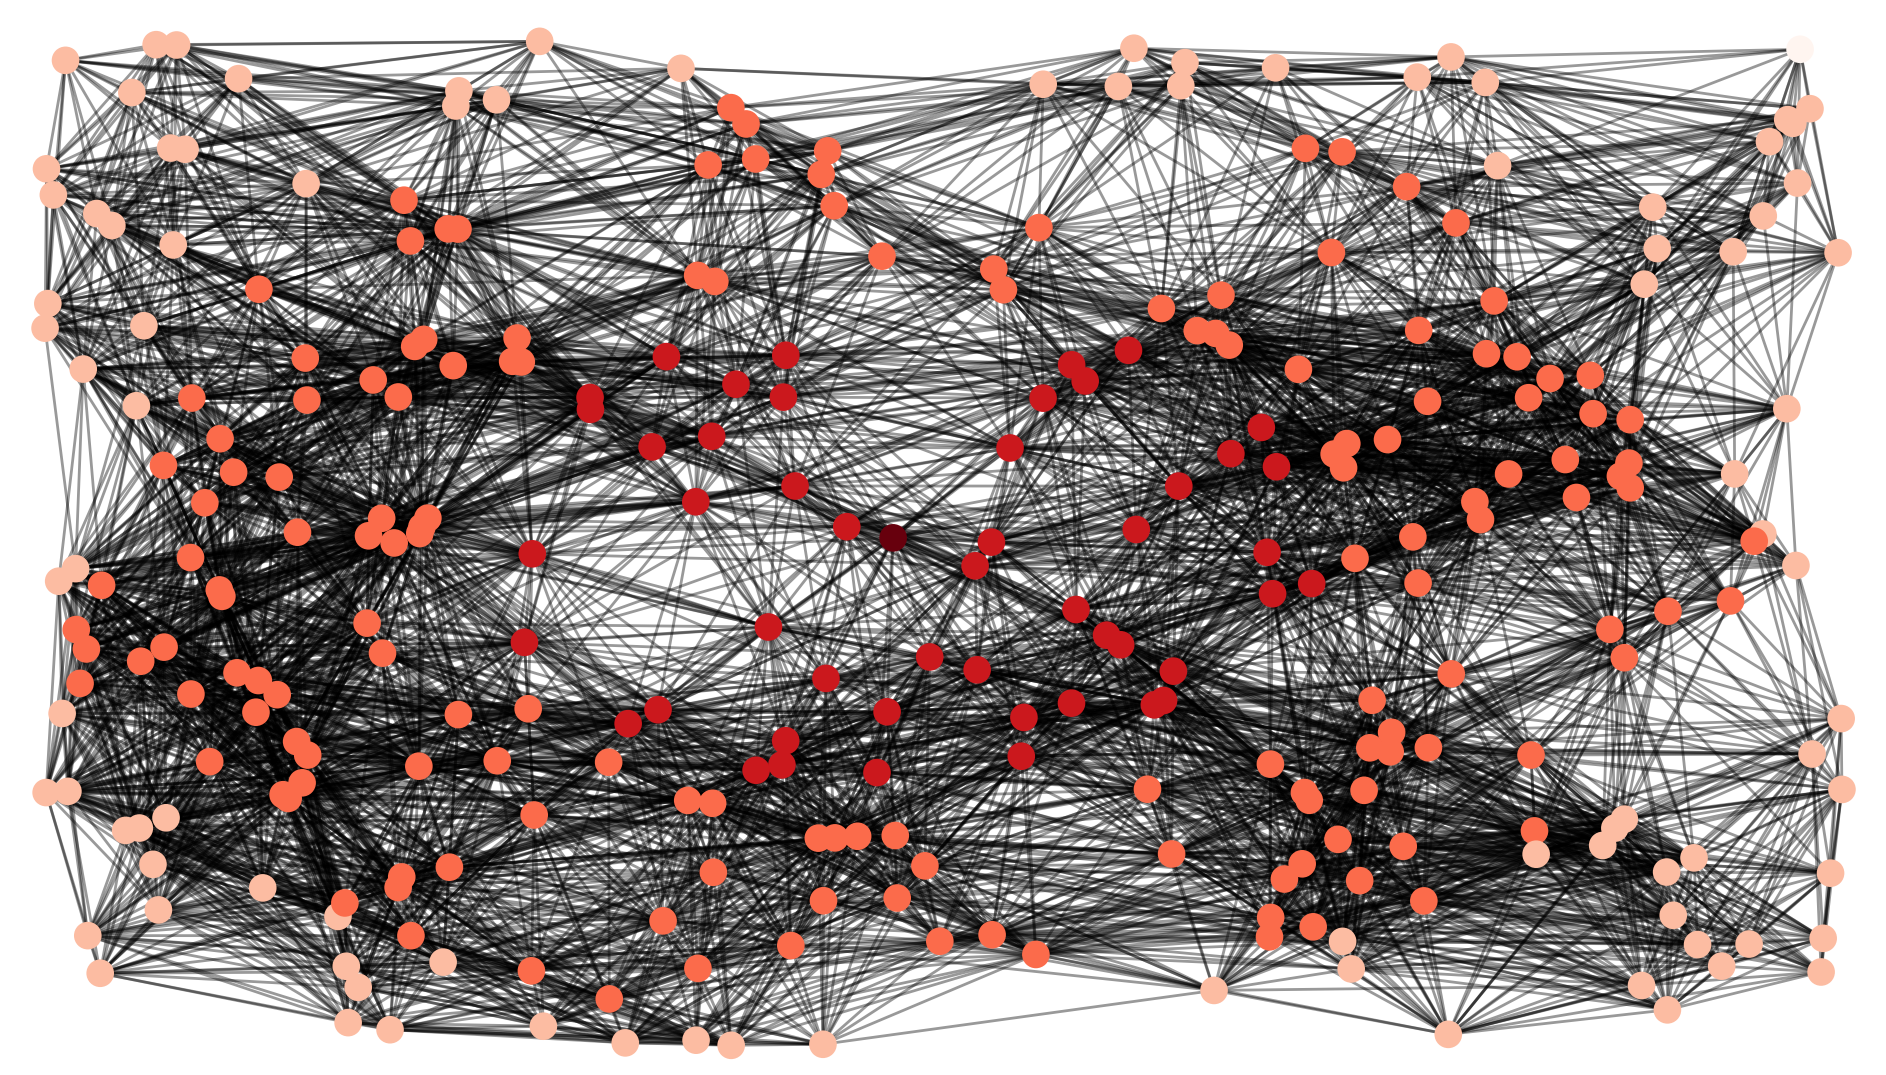
\includegraphics[width=0.7\linewidth]{Experiments/figures/network_image.png}
  \end{tabular}
  \caption{\label{fig:synthetic_weights} Markov Random Fields
    generated by data and algorithm described in section~\ref{sec:con_stock_graph}.}
\end{figure*}




%%% Local Variables:
%%% mode: latex
%%% TeX-master: "../thesis"
%%% End:
